\problemname{Free food}
Hsara loves free food.

Tonight Hsara is going out for a dinner at a restaurant with his organisation and Hsara is thinking about the chances of someone else paying for the dinner. Exactly one person will pay for the entire dinner (everyone's food), but not any person. It is only allowed to pay for dinner if no supperior (possibly indirect, for example, your boss' boss) in the organisation is present at the table.

The organisation consists of $N$ people numbered from $1$ to $N$. Each person, except for the CEO, has exactly one boss. Given each person's boss and a list of people present at the table, determine how many people are able to pay for the dinner.

\begin{figure}[h!]
	\begin{center}
		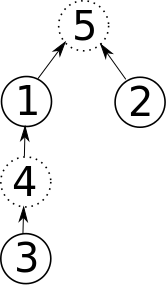
\includegraphics[width=0.2\textwidth]{tree.png}
		\caption{Illustration of the organisation in the first sample.}
	\end{center}
\end{figure}


\section*{Input}
The first line consists of two integers, $N$ - the number of people in the organisation and $1 \le M \le N$ - the number of people at the table.

The second line consists of $N$ integers. The $i$:th integer is the boss of person $i$. 0 means that person $i$ is the CEO. There will be exactly one CEO.

The third line consists of $M$ integers indicating the people present at the table.

\section*{Output}
Print an integer - the number of people at the table who would be able to pay for the dinner.

\section*{Grading}
Your solution will be tested on several groups of test cases. To get points for a group you need to pass all the tests of that group.

\begin{tabular}{| l | l | l |}
	\hline
	Group & Points & Constraints \\ \hline
  1     & 49         & $2 \le N \le 2\,000$ \\ \hline
  2     & 51         & $2 \le N \le 100\,000$. \\ \hline
\end{tabular}

\section*{Explanation}
In the first sample person 1 and person 2 can pay. Person 3 can't pay because person 1 is at the table.

In the second sample person 5 is the CEO and at the table. Therefore only person 5 can pay.
